\chapter{Спектральный анализ коротких всплесков Конус-Винд} \label{sGRB_spectral_catalog}
Настоящая глава посвящена спектральному анализу 296 коротких всплесков Конус-Винд (\textit{KW}),
локализации которых была описана в Главе~\ref{IPN_catalog}.

\section{Методика}
Для каждого всплеска на основе его локализации вычислялась матрица отклика детектора
(см. Главу~\ref{KW_description}).
Типичный спектр короткого гамма-всплеска по данным \kws состоит из подгруппы первых 
четырех спектров с временем накопления 64~мс на интервале 
от 0 до 0.256~с относительно триггера. Около 10\% всплесков имеют значимое 
излучение в пятом спектре (0.256--8.192~с). В примерно для 4\% ярких событий
границы интервалов накопления спектров с 5-го и далее были изменены системой адаптации.

Спектр фона для коротких всплесков без продлённого излучения, как правило, 
брался на интервале $T_0+25$~с со временем накопления около 100~с.
Калибровка аппаратного спектра производилась по фоновому спектру.
Для примерно четверти всплесков анализ многоканальных спектров был не возможен, из-за того 
что основная часть события лежала до начала измерения спектров. 
Для такого всплеска строился трехканальный спектр, с использованием отсчетов временной истории, 
накопленных за полную длительность всплеска $T_{100}$.
Набор спектров содержит 216 многоканальных интегральных спектров и 78~--- трехканальных. 

Из-за малого числа отсчётов (количества фотонов) для большинства всплесков 
пиковый поток определялся на основе интегрального спектра. 
Только для 18 достаточно интенсивных событий можно было выделить спектр вблизи 
максимальной скорости счёта.
Итоговой набор спектров состоял из 216 интегральных многоканальных спектров 
(без учёта 18 спектров вблизи пиковой скорости счёта) и 78 трёхканальных. 
Два слабых всплеска: GRB19960325\_T69892 и GRB19980614\_T31854 имели сбои во 
временных историях и спектрах и были исключены из рассмотрения.

\subsection{Многоканальные спектры}
Процедура определения спектральных параметров, описанная в Главе~\ref{KW_description}, 
для многоканальных спектров производилась в программе 
\texttt{XSPEC}\citep{Arnaud_1996ASPC} версии~12.8.0.
Для определения параметров моделей использовалась статистика $\chi^2$. 
Спектральные каналы были сгруппированы по не менее 10 отсчётов на канал для обеспечения 
близкой к гауссовой статистики отсчётов. Группировка по не менее 20 отсчётов на канал 
приводила к исключению из процесса моделирования спектра старших каналов, 
что в некоторых случаях значительно сужало энергетический диапазон. 
В качестве нормировки модели использовался поток в диапазоне 10~кэВ--10~МэВ, 
который вычислялся с использованием модели \texttt{cflux} в \texttt{XSPEC}.
Ошибки спектральных параметров определялись на основе $\Delta \chi^2 = 1$ и $2.706$ для уровней 
значимости 68\% и 90\%, соответственно.

Для каждой описанной выше модели определялись параметры, наиболее подходящая 
модель выбиралась на основе различия $\chi^2$ между моделями. Критерием для предпочтения
модели с одним дополнительным параметром было $\Delta \chi^2 \geq 5$ с соответствующей 
вероятностью $\approx 0.025$. Было обнаружено, что такое значение предпочтительно 
для нашего набора всплесков по сравнению с часто используемым $\Delta \chi^2 \geq 6$,
так как оно даёт значительно меньше расходящихся PL моделей, в качестве наилучших,
что критично для вычисления энергетики всплесков.

\subsection{Трёхканальные спектры}
Определение параметров PL и CPL моделей для 78 трёхканальных спектров производилось 
специально созданной программой. При этом ошибки параметров определялись методом Монте-Карло
для 400 реализаций исходных спектров.

Для проверки методики мы сравнили результаты многоканального и трёхканального спектрального анализа
на наборе 216 всплесков с многоканальными спектрами.
Для каждого всплеска был взят  трёхканальный спектр, накопленный в течение 
интервала измерения многоканального спектра.
Затем сравнивались параметры модели, которые лучше всего описывают многоканальный спектр
с параметрами и той же модели, полученными по трёхканальному спектру.
В случае PL полученные фотонные индексы согласуются для двух типов
спектрального анализа. Для CPL мы обнаружили, что  $\alpha$ также в целом
согласуется между двумя типами спектров. То же самое верно и для $E_\rmn{p}$, но
только в случае если значение попадает в энергетический диапазон трёхканального спектра
($\lesssim 1$~МэВ), в противном случае трёхканальный анализ давал завышенную и 
плохо ограниченное значение $E_\rmn{p}$. Это показывает, что на основе данных \kws 
можно получать достаточно точные значения спектральных параметров и энергетики
даже когда многоканальные спектральные данные отсутствуют.

Поскольку аппроксимация трёхканального спектра моделью CPL имеет нулевое число степеней свободы
(и, в случае сходимости, $\chi_\rmn{CPL}^2=0$), наиболее подходящая модель 
не может быть выбрана на основе критерия $\Delta \chi^2 \geq 5$.
Поэтому, для того чтобы не переоценить энергетику всплеска, для вычисления $S$ и $F_\rmn{peak}$
использовалась модель CPL в случаях когда $E_\rmn{p}$ была ограничена снизу.

\section{Результаты}
\subsection{Спектральные параметры}
Статистика наилучших моделей для интегральных спектров: CPL~--- 203 GRBs, BAND~--- 9 GRBs и PL~---~4.
Так как ни один метод основанный на использовании функции правдоподобия не даёт 
вероятности того, что конкретная модель является единственной моделью, 
правильно описывающей данные, в каталоге также рассматриваются все 
модели параметры которых ограничены.

Для моделей CPL и BAND требовалось чтобы и $\alpha$ и $E_\rmn{p}$ имели ограниченные ошибки,
и для модели BAND дополнительно требовалось $\beta > -4$. Для исключения моделей
с большими невязками дополнительно было наложено условие на вероятность 
случайного получения заданного значения статистики $\chi^2$ 
(вероятностью нулевой гипотезы) $P> 10^{-6}$.

Результаты спектрального анализа приведены в Таблице~\ref{tab:spec_par}.
Таблица содержит десять колонок со следующей информацией: 
(1) обозначение всплеска (см. Таблицу~\ref{tab:info});
(2) тип спектра, `i' обозначает, что спектр интегральный и использовался для вычисления $S$,
 `p' означает, что спектр измерялся вблизи пиковой скорости счёта и использовался 
для вычисления $F_\rmn{peak}$, или для вычисления обоих значений `i,p';
колонки (3) и (4) содержат время начала измерения спектра $T_\rmn{start}$ (относительно $T_0$) 
и время накопления спектра $\Delta T$;
(5) содержит список моделей с ограниченными параметрами (наилучшая модель отмечена);
(6)--(8) содержат низкоэнергетический фотонный индекс $\alpha$, высокоэнергетический фотонный индекс $\beta$, 
и $E_\rmn{p}$;
(9) нормализация (энергетических поток в диапазоне 10~кэВ--10~МэВ);  
(10) $\chi^2/\rmn{dof}$ и вероятность нулевой гипотезы $P$.
В случае если нижний предел на $\beta$ не определён в таблице приведено значение
$\beta_\rmn{min} - \beta$, где $\beta_\rmn{min}=-10$~--- нижний предел параметра,
используемый при аппроксимации. Суммарно таблица содержит параметры 479 моделей
для интегральных спектров (212~--- CPL, 118~--- BAND, and 149~--- PL)

Таблица~\ref{tab:spec_par_3ch} содержит результаты полученные для 78 трёхканальных спектров. 
Для всех всплесков кроме одного преведены параметры модели CPL, для GRB19961113\_T80522 с 
неограниченной $E_\rmn{p}$ приведены параметры модели PL. 
Восемь колонок таблицы содержат следующую информацию: 
(1) обозначение всплеска (см. Таблицу~\ref{tab:info});
колонки (2) и (3) cсодержат время начала измерения спектра $T_\rmn{start}$ (относительно $T_0$) 
и время накопления спектра $\Delta T$;
(4) спектральная модель; 
колонки (5) и (6) содержат $\alpha$ и $E_\rmn{p}$, соответственно;
(7) нормализация (энергетических поток в диапазоне 10~кэВ--10~МэВ); 
(8) $\chi^2/\rmn{dof}$.

На Рис.~\ref{fig:par_dist}, представлено распределение интегральных спектров по $E_\rmn{p}$ и $\alpha$.
Фотонные индексы $\alpha$ наиболее подходящих спектральных моделей распределены 
вокруг значения~$-0.5$. 
Около 66\% фотонных индексов $\alpha > -2/3$, нарушают <<линию смерти>> для 
синхротронной модели излучения~\citep{Preece_1998ApJL}, в тоже время только около 
1\% (три фотонных индекса для PL моделей) фотонных индексов $\alpha< -3/2$, 
нарушают предел охлаждения в синхротронной модели излучения \textbf(Раскрыть смысл этих пределов). 
Для четырёх спектров, которые описываются степенной моделью, фотонные индексы 
находятся на мягком конце распределения $\alpha$. Для 9-и моделей BAND индексы $\beta$
распределены вблизи значения $-2.3$.
Распределение по $E_\rmn{p}$ для CPL моделей имеет максимум около 500~кэВ 
и покрывает около двух порядков величины. 
Было исследовано различие значений $E_\rmn{p}$ между моделями BAND и CPL в наборе 
моделей с ограниченными параметрами и было обнаружено, что для каждого спектра значения согласуются
в пределах ошибок на уровне 90\%.

\subsection{Всплески с дополнительной спектральной компонентой}
Для трёх ярких всплесков было получено $P<0.001$ для интегральных спектров. 
Детальное рассмотрение этих всплесков выявило причину малых значений $P$.
Всплеск GRB20060306\_T55358, с $P \approx 10^{-4}$, демонстрирует сильную 
спектральную эволюцию~--- жесткость спектра уменьшается в течении всплеска, 
что приводит к плохой аппроксимации интегрального спектра моделями BAND и CPL.
Однако, эти модель BAND хорошо описывают ($P>0.05$) отдельные спектры этого яркого всплеска.
Было обнаружено, что интегральные спектры двух других всплесков GRB19960908\_T25028 и GRB20031214\_T36655
хорошо описываются суммой функций CPL и PL.
Помимо перечисленных всплесков явные систематические отклонения модели от спектра
были обнаружены для интегрального спектра GRB19980205\_T19785 ($P=0.08$), 
этот спектр также хорошо аппроксимируется суммой CPL+PL.
 
Параметры CPL+PL аппроксимаций интегральных спектров описанных всплесков приведены в Таблице~\ref{tab:extra_comp}. 
Степенная компонента этих спектров, которая также детектируется в большинстве отдельных спектров,
является достаточно жесткой ($\alpha \sim -2$), даёт основной вклад в спектр на  
энергиях ниже $\sim 50$--100~кэВ.
Жесткая CPL компонента имеет $E_\rmn{p}\sim(1.5\textrm{--}2)$~МэВ и достаточно пологий
фотонный индекс $\alpha > -1$).
Все перечисленные всплески находятся среди 10\% наиболее интенсивных всплесков
в смысле интегральных энергетических потоков, при этом
GRB20031214\_T36655 и GRB20060306\_T55358 имеют наибольшие потоки в наборе.

\subsection{Интегральные и пиковые потоки}
Значения $S$ и $F_\rmn{peak}$ вычислялись с использованием энергетического потока,
полученного для наиболее подходящей спектральной модели в диапазоне 10~кэВ--10~МэВ.
Так как интервал накопления спектра обычно отличался от $T_{100}$, применялась 
коррекция, которая учитывала излучение лежащие вне интервала накопления спектра 
для вычисления $S$.
Для коротких всплесков с продлённым излучением интегральные энергетические потоки 
вычислялись отдельно для EE и начального импульса (см. Раздел~\ref{sec:EE}).
Значение $F_\rmn{peak}$ вычислялось на масштабе 16~мс с использованием наиболее 
подходящей спектральной модели для спектра вблизи максимальной скорости счёта.
Для получения $F_\rmn{peak}$ поток по модели умножался на отношение 
пиковой скорости счёта на масштабе 16~мс к средней скорости счёта за интервал 
накопления спектра. Обычно для коррекции использовались отсчёты в группах каналов
G2+G3, G1+G2 только G2 или G1+G2+G3 в зависимости от жесткости спектра.

В таблице~\ref{tab:fl_pf} приведены значения $S$ и $F_\rmn{peak}$ для 294 всплесков.
В первой колонке дано обозначение всплеска (см. Таблицу~\ref{tab:info})
Три последующие колонки содержат $S$; время начала 16~мс интервала, содержащего
пиковую скорость счёта в диапазоне G2+G3; и $F_\rmn{peak}$.
Распределения всплесков по $S$ and $F_\rmn{peak}$ показаны на рисунке~\ref{fig:fl_pf_dist}.


\subsection{Короткие всплески с продлённым излучением}
Продлённое излучение (EE), которое наблюдается после короткого начального импульса (IP),
наблюдалось у некоторой части коротких всплесков, зарегистрированных различными экспериментами:
\textit{CGRO}-BATSE~\citep{Burenin_2000AstL, Norris_and_Bonnel_2006ApJ, Bostanci_2013MNRAS}, 
KW~\citep{Mazets_2002astroph, Frederiks_2004ASPC}, 
\textit{INTEGRAL}-SPI-ACS~\citep{Minaev_2010AstL}, 
\textit{Swift}-BAT~\citep{Norris_2011ApJ, Sakamoto_2011ApJS}, 
и \textit{Fermi}-GBM~\citep{Kaneko_2015MNRAS}. 
Поиск кандидатов в короткие всплески с EE был произведён в Главе~\ref{KW_GRB_classification}.
Только для 22-х событий с ярким EE были проанализированы его многоканальные спектры.
Здесь приводятся результаты спектрального анализа продлённого излучения.

%We defined the following search criteria: 
%the burst initial pulse should meet our criteria for a short GRB, i.e. have $T_{50}<0.6$~s;
%and the remaining part of burst (EE) shouldn't exhibit peaks with prominent spectral evolution. 
%Applying these criteria to the full KW sample, we found 31 short GRBs with EE candidates. 
%Only for 22 events EE was bright enough to allow spectral analysis.
%The initial pulses of these events are classified in Table~\ref{tab:durations} as Iee or Iee/II.

В таблице~\ref{tab:EE} приведены параметры EE. Десять колонок содержат следующие параметры:
(1) обозначение всплеска (см. Таблицу~\ref{tab:info});
колонки (2) и (3) содержат время начала EE (относительно $T_0$) и его длительность, 
вычисленную на уровне значимости $5\sigma$ в диапазоне G2 или G2+G1;
колонки (4) и (5) содержат время начала измерения спектра $T_\rmn{start}$ (относительно $T_0$) 
и его время накопления $\Delta T$;
(6) наиболее подходящая модель для каждого спектра;
(7) и (8) содержат $\alpha$ и $E_\rmn{p}$;
(9) интегральный энергетический поток в диапазоне 10~кэВ--10~МэВ; 
(10) $\chi^2/\rmn{dof}$ и вероятность нулевой гипотезы $P$.

Для 16 всплесков наилучшей спектральной моделью для EE является PL и для 6~--- CPL.
Фотонные индексы модели PL находятся в диапазоне от $-2.7$ до $-1.3$ с медианой $-1.6$,
и в диапазоне от $-1.6$ до $-0.2$ с медианой $-1.2$ для модели CPL.
Значения $E_\rmn{p}$ находятся в диапазоне от $160$~кэВ до $\sim 1.5$~МэВ с медианой $300$~кэВ
и средним геометрическим $350$~кэВ. Наибольшее значение $E_\rmn{p}\approx 1.5$~МэВ 
было получено для всплеска GRB20070207\_T75644 обладающего на порядок более интенсивным EE,
чем у остальных всплесков.
Для указанных 22-х всплесков было вычислено отношение потоков EE/IP, 
которое изменяется в пределах от 0.05 до $\approx 15$ с медианой 5.0 и средним 
геометрическим 2.8. Для GRB20070207\_T75644 это отношение составляет $\approx 750$.

Из шести всплесков, у которых EE описывается моделью CPL, у четырёх $E_\rmn{p}$ EE 
меньше чем у начального импульса и для двух всплесков наблюдается обратная ситуация:
для GRB19950526\_T16613 с $E_\rmn{p} = 296(-68,+118)$~keV в начальном импульсе и 
$E_\rmn{p}= 489(-125,+230)$~keV в EE; и для упомянутого ранее GRB20070207\_T75644.

\section{Обсуждение результатов}
В главе представлены результаты спектрального анализа 294-х коротких гамма-всплесков,
зарегистрированных в эксперименте Конус-Винд, этот набор составляет $\sim 15$\% 
от полного числа всплесков, зарегистрированных за первые 15 лет работы инструмента.
Набор включает $\sim 70$\% всплесков Типа~I, $\sim 8$\% Типа~II и $\sim 12$\%
имеют неопределённый тип (I или~II). Доля коротких всплесков с продлённым 
излучением составляет $\sim 10$\%.

Суммарно было проанализировано 256 многоканальных спектров: 216 интегральных,
18 пиковых и 22 спектра продлённого излучения; и 78 трёхканальных спектров.
Таблица~\ref{tab:pardist} содержит медианы и 90\% интервалы распределений спектральных
параметров и энергетики, полученных в главе. В первой колонке дано название параметра;
во второй тип спектральных данных: многоканальный или трёхканальный спектр;
последующие колонки содержат медианы и 90\% интервалы для распределений
$\alpha$, $\beta$, $E_\rmn{p}$, $S$ и $F_\rmn{peak}$.

Результаты анализа сопоставлялись ранее полученными результатами для коротких всплесков 
\textit{Fermi}-GBM~\citep{Gruber_2014ApJS} и \textit{CGRO}-BATSE~\citep{Goldstein_2013ApJS}.
Полученные в главе результаты согласуются с результатами других экспериментов в том,
что большая часть коротких всплесков описывается моделью CPL с жесткими $\alpha \sim -0.5$
и $E_\rmn{p}$ в диапазоне 100~кэВ--2~МэВ.
Число многоканальных спектров, описываемых моделью BAND составляет $\sim 4$\% от 
коротких всплесков \kws с многоканальными спектрами, такое же соотношение наблюдается
для других инструментов. Среди 5\% событий с наибольшим $S$, доля интегральных спектров,
описываемых моделью BAND составляет 20\% (три из 15 всплесков), для большинства остальных
$\beta$ ограничена сверху значением $\sim -2.5$. Это свидетельствует в пользу того,
что отсутствие наблюдаемого степенного поведения спектра коротких всплесков в области больших
энергий связано с природой источника, а не вызвано малой статистикой отсчётов. 

В данной работе не ставилась задача проверки применимости более сложных моделей
для описания спектров коротких всплесков.
Однако, среди 216 всплесков с многоканальными спектрами было обнаружено три
события, для описания которых необходима дополнительная жесткая степенная 
спектральная компонента с фотонным индексом $\sim -2$. Эти всплески входят в 10\%
наиболее интенсивных событий из набора. Отношение энергетических потоков PL
компоненты к CPL находится в диапазоне от 0.03 для GRB20031214\_T366655 до
0.4 для GRB19980205\_T19785. Обнаруженная компонента может иметь ту же природу,
что и обнаруженная в GRB~081024B~\citep{Abdo_2010ApJ_712_558A} и 
GRB~090510~\citep{Ackermann_2010ApJ_716_1178A} на основе данных \textit{Fermi}~GBM и~LAT.
GRB~081024B не был зарегистрирован \kws триггерном режиме, GRB~090510 (GRB20090510\_T01381)
содержится в нашем наборе. Для описания спектра последнего всплеска степенная 
компонента не требуется, верхний предел на поток степенной компоненты с фотонным 
индексом $-1.7$ составляет $\sim 1 \times 10^{-6}$~эрг~см$^{-2}$~с$^{-1}$ для 
уровня значимости 90\%. Соответствующий предел на отношение потока PL компоненты 
к потоку в основной компоненте составляет $\lesssim 0.02$ на уровне значимости 90\%.
\textbf{Написать подробней про эти всплески, добавить картинки.}

Было обнаружено, что 31 всплеск из набора 1939 \kws гамма-всплесков зарегистрированных
с 1994 по 2010 год могут быть классифицированы как короткие всплесков с EE, 
основываясь на длительности начального импульса и отсутствие в последующием излучении 
заметной спектральной эволюции. Из них, 21 всплеск имеет интенсивность EE достаточную
для анализа многоканальных спектров. Для семи из нэтих всплесков спектр EE описывается
моделью с изломом (CPL), то же было обнаружено для двух из 19 всплесков BATSE~\citep{Bostanci_2013MNRAS}
и для четырёх из 14 всплесков GBM~\citep{Kaneko_2015MNRAS}.
Набор коротких всплесков с продлённым излучением \kws включает два всплеска, 
где EE наблюдалось на BATSE, и три, где EE наблюдалось GBM. Результаты спектрального
анализа этих всплесков по данным \kws согласуются с результатами упомянутых инструментов.

Хотя начальный импульс GRB20070207\_T75644 удовлетворяет критерию короткого всплеска,
наличие очень интенсивного и жесткого излучения с $E_\rmn{p} \sim 1.5$~МэВ, 
изначально классифицированного как EE, свидетельствует в пользу того, что это
длинный всплеск с коротким прекурсором с $E_\rmn{p} \sim 300$~кэВ.
 
Яркий близкий всплеск GRB~060614, который был классифицирован как короткий 
всплеск с EE~\citep{Gehrels_2006Nature} был зарегистрирован \kws ($T_0$(KW)=45831.590~с;~\citep{Golenetskii_GCN5264}).
Этот всплеск не был включён в наш набор коротких всплесков из-за большой 
длительности начального импульса$T_{50}=2.7 \pm 0.3$~с.

Яркий начальный импульс гигантской вспышки (GF) источника мягких повторяющихся гамма-всплесков, 
произошедшей в близкой галактике, может выглядеть в данных гамма детектора как короткий гамма-всплеск. 
Верхней предел на частоту GF на основе локализаций коротких свсплесков \kws был
получен в главе~\ref{SGR_GF_search}. При этом было обнаружено только два кандидата:
GRB~051103 (GRB20051103\_T33943) в группе галактик M81/M82~\citep{Frederiks_2007AstLett} и 
GRB~070201 (GRB20070201\_T55390) в галактике M31~\citep{Mazets_2008ApJ}.
Оба события находятся среди 10\% наиболее интенсивных событий на основе интегрального 
энергетического потока. Спектральные параметры всплесков являются типичными для 
набора коротких всплесков KW.

Избыток отсчётов, наблюдаемый вплоть до 90~с после триггера GRB~070201, 
был интерпретирован как хвост гигантской вспышки~\citep{Mazets_2008ApJ}.
Значимость избытка составляет $4.3\sigma$, поэтому он не был обнаружен при 
поиске продлённого излучения (с порогом $5\sigma$).

На рис.~\ref{fig:EpT50} показано соотношение $E_\rmn{p}$, для наиболее подходящей CPL модели,
и длительности всплеска $T_{50}$. Всплески Типа~I, в среднем, короче и жестче 
($E_\rmn{p}\gtrsim 200$~кэВ), чем всплески Типа~II, что подтверждает классификацию,
полученную на основе распределения жесткость-длительность.
Среди 4-х всплесков описываемых моделью PL, два всплеска принадлежат к типам I и II,
и два имеют неопределённый тип (I/II). Явный недостаток всплесков с $E_\rmn{p}\lesssim 100$~кэВ,
скорее всего связан с эффектом селекции. 
Распределение по длительности начальных импульсов коротких всплесков типа~I с EE (Iee) согласуется с 
распределением для обычных коротких всплесков типа~I, о чем свидетельствует значение p-значения
теста Колмогорова-Смирнова $P_\rmn{KS}=0.5$. Также было обнаружено, что
начальные импульсы всплесков типа Iee, в среднем, жестче ($E_\rmn{p}$ в $\sim 1.5$ раза выше),
чем всплески типа~I ($P_\rmn{KS} = 0.01$). В заключении были сопоставлены распределения 
всплесков типов Iee и~I по $S$ и $F_\rmn{peak}$, для пар распределений 
была получена $P_\rmn{KS} \sim 0.01$, что свидетельствует о различие распределений,
при этом всплески с EE, в среднем, более интенсивные.

На рис.~\ref{fig:EpvsFPandFL} приведены соотношения $E_\rmn{p}$ с $S$ и $F_\rmn{peak}$.
Распределение 78 слабых всплесков с трёх-канальными спектрами по спектральным параметрам 
и $F_\rmn{peak}$ схоже с более интенсивными событиями, эти всплески являются продолжением
распределения коротких/жестких (Тип~I) всплесков в область низких $S$  на диаграмме $E_\rmn{p}$--$S$.
Явным выбросом из  $E_\rmn{p}$--$F_\rmn{peak}$ распределения является предполагаемая 
GF в галактике M31, что подкрепляет свидетельства в пользу отличной от GRB природы этого события.

Всплески типов I и~II занимают практически не пересекающиеся области на диаграмме $E_\rmn{p}$--$S$.
Всплески типа~I образуют вытянутое распределение, которое, в среднем, подчиняется 
соотношению $E_\rmn{p} \propto S^{1/2}$. Всплески типа II образуют небольшую группу событий
с низкой $E_\rmn{p}$, которая представляет собой малую часть распределения длинных всплесков.
На плоскости $E_\rmn{p}$--$F_\rmn{peak}$ всплески типа~II продлевают корреляцию 
жесткость-интенсивность в область низких $E_\rmn{p}$ и малых $F_\rmn{peak}$.
Так как только для девяти всплесков из набора были определены космологические 
красные смещения ($z\sim 0.1$--1.0, определённые как спектрометрически, так и
фотометрически), свойства всплесков в собственной системе отсчёта здесь не обсуждаются.
Хотя инструментальные эффекты селекции влияют на параметры представленного набора,
корреляции наблюдаемых параметров всё же могут отражать корреляции параметров 
в системе отсчёта источника всплеска $E_\rmn{p,rest}$--$E_\rmn{iso}$~--- 
соотношение Амати~\citep{Amati_2002AandA} и $E_\rmn{p,rest}$--$L_\rmn{iso}$~--- 
соотношение Йонетоку~\citep{Yonetoku_2004ApJ}
(см., к примеру, работу~\citep{Nava_2008MNRAS} и ссылки в ней).
Таким образом, описанные свойства распределения жесткость-интенсивность 
в системе наблюдателя, полученные для всплесков типов I и II из набора коротких 
всплесков KW, свидетельствуют в пользу того, что короткие/жесткие всплески подчиняются 
своему соотношению Амати на плоскости $E_\rmn{p,rest}$--$E_\rmn{iso}$
(см., к примеру, работу~\citep{Nava_2011MNRAS} и ссылки в ней).

Интегральные распределения $\log N$--$\log S$ и $\log N$--$\log F_\rmn{peak}$
для набора 294 коротких всплесков KW, а так же степенные распределения с индексом $-3/2$, 
соответствующие однородному распределению источников всплесков в пространстве,
представлены на рис.~\ref{fig:logNlogS_PF}.
Распределение $\log N$--$\log S$ следует однородному распределению в небольшой 
области интегральных потоков $(\sim 4\textrm{--}10)\times 10^{-6}$~эрг~см$^{-2}$.
В то время как недостаток слабых всплесков может быть объяснён эффектами селекции,
явный избыток интенсивных всплесков $S \gtrsim 10^{-5}$~эрг~см$^{-2}$ требует
дальнейшего анализа.
В заключении, распределение $\log N$--$\log F_\rmn{peak}$ коротких всплесков \kws,
по видимому, имеет более пологий степенной индекс. Для $F_\rmn{peak}$ в диапазоне 
$(0.2\textrm{--}8.5)\times 10^{-5}$~эрг~см$^{-2}$~с$^{-1}$, для интегрального распределения 
был получен степенной индекс $-1.16 \pm 0.01$ ($\chi^2_r = 1.2$).

\section{Заключение}
В данной главе представлен спектральный анализ коротких гамма-всплесков Конус-Винд.

По результатам этой главы выносятся на защиту следующие результаты:
\begin{enumerate}
\item Каталог с результатами спектрального анализа 296 коротких гамма-всплесков Конус-Винд;
\item Обнаружение дополнительной спектральной компоненты у трёх коротких всплесков Конус-Винд.
\end{enumerate}

Результаты отражены в публикации \\
D.~S.~Svinkin, D.~D.~Frederiks, R.~L.~Aptekar, et al. Konus-\textit{Wind} catalog of short GRBs //
to be submitted to ApJS

Автор лично произвел спектральный анализ описанного набора коротких гамма-всплесков.
Интерпретация результатов была сделана совместно с соавторами при активном участии автора.


\begin{figure}
    \begin{center}
        \includegraphics[width=0.75\textwidth]{gHRvsT50_ru.eps}
    \end{center}
    \caption{
    Соотношение жесткость длительность для 1143 якких всплесков \kws (серые точки).
    Распределение моделировалось суммой двух двумерных гауссовых распределений
    EM-алгоритмом (\textit{Expectation-maximization (EM) algorithm}). 
    Контуры обозначают уровни вероятности $1\sigma$, $2\sigma$ и $3\sigma$ для каждой
    гауссовой компоненты. Вертикальная пунктирная линия обозначает границу ($T_{50}=0.6$~с)
    между короткими и длинными всплесками \kws. Типы всплесков с $T_{50}<0.6$~с 
    обозначены цветами.
    \label{fig:HRvsT50}}
\end{figure}

\begin{figure}
	\begin{center}
		\subfigure[]{\label{falpha}\includegraphics[height=0.45\textwidth]{gDistAlpha_ru.eps}}
		\subfigure[]{\label{fEp}\includegraphics[height=0.45\textwidth]{gDistEp_ru.eps}}
	\end{center}
    \caption{
    Распределение $\alpha$~\subref{falpha} и $E_\rmn{p}$~\subref{fEp}, полученных 
    в результате моделирования интегральных спектров. Распределение для каждой модели
    показано отдельно.
    \label{fig:par_dist} }
\end{figure}


\begin{figure}
	\begin{center}
		\subfigure[]{\label{ffl}\includegraphics[height=0.45\textwidth]{gDistS_ru.eps}}
		\subfigure[]{\label{fpf}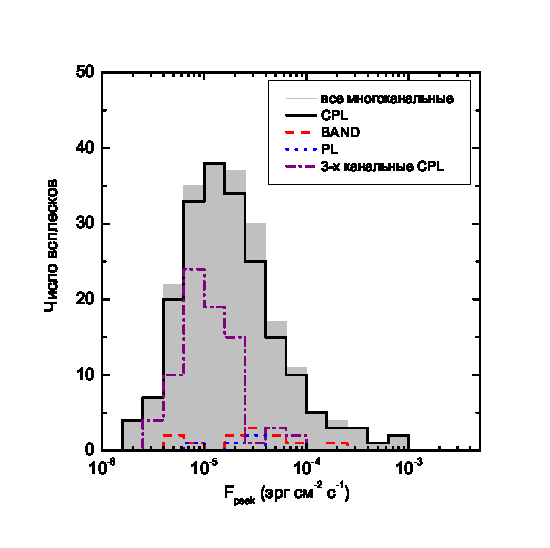
\includegraphics[height=0.45\textwidth]{gDistPF_ru.eps}}
	\end{center}
\caption{
    Распределение интегральных~\subref{ffl} и пиковых энергетических потоков~\subref{fpf}
    Серым на каждой панели показано суммарное по всем моделям распределение для 216
    многоканальных спектров, распределения для каждой модели показаны отдельно. 
    Штрихпунктирной линией показаны распределения для 78 трёхканальных спектров.
    \label{fig:fl_pf_dist} }
\end{figure}

\begin{figure}
	\begin{center}
		\subfigure[]{\label{fEpTypeII}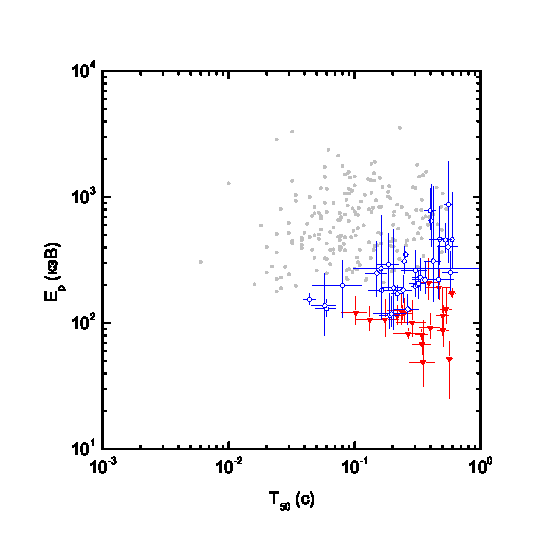
\includegraphics[height=0.45\textwidth]{gEpvsT50TypesII_ru.eps}}
		\subfigure[]{\label{fEpEEip}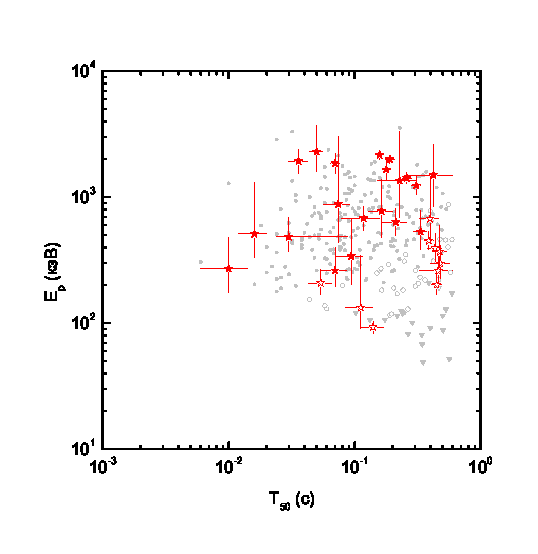
\includegraphics[height=0.45\textwidth]{gEpvsT50ipEE_ru.eps}}
	\end{center}
\caption{
    Соотношение $E_\rmn{p}$ и $T_{50}$ (только для модели CPL).
    На панели~\subref{fEpTypeII} показаны всплески типа~I (серые точки), типа~II (красные треугольники)
    и всплески неопределённого типа, I или~II (синие окружности).
    На панели~\subref{fEpEEip} показаны всплески типа~I с EE (заполненные красные звёзды)
    и всплески неопределённого типа Iee или~II (пустые красные звёзды)
    Для всплесков типа~I ошибки не показаны. 
    \label{fig:EpT50}}
\end{figure}

\begin{figure}
	\begin{center}
		\begin{minipage}[t]{1\textwidth}
		\subfigure[]{\label{fig:EpFluence}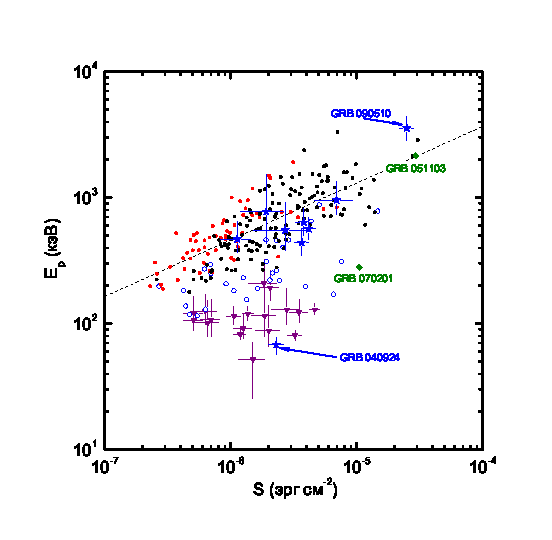
\includegraphics[width=0.5\textwidth]{gEpvsFl_ru.eps}}
		\subfigure[]{\label{fig:EpFluence_EE}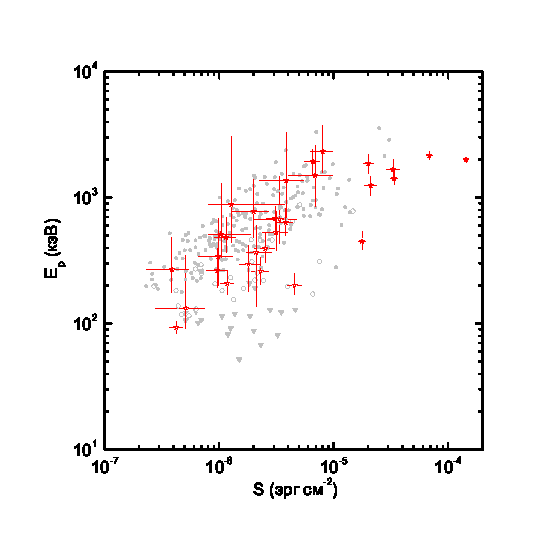
\includegraphics[width=0.5\textwidth]{gEpvsFlEE_ru.eps}}
        %\vspace{-0.5cm}
		\end{minipage}
		\begin{minipage}[t]{1\textwidth}
		\subfigure[]{\label{fig:EpPF}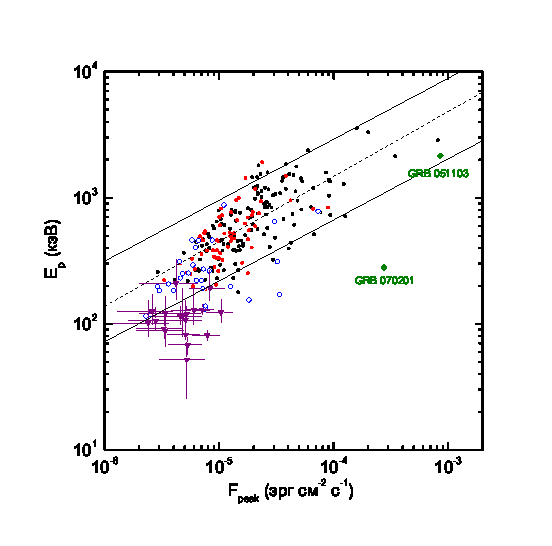
\includegraphics[width=0.5\textwidth]{gEpvsPF_ru.eps}}
		\subfigure[]{\label{fig:EpPF_EE}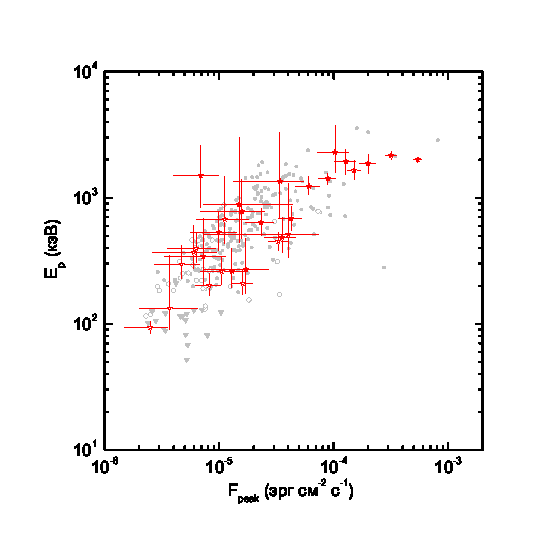
\includegraphics[width=0.5\textwidth]{gEpvsPFEE_ru.eps}}
        %\vspace{-0.5cm}
		\end{minipage}
	\end{center}
\caption{
    Соотношение $E_\rmn{p}$ с $S$ и $F_\rmn{peak}$ для всплесков, описываемых моделью CPL.
    На панели~\subref{fig:EpFluence} показано соотношение $E_\rmn{p}$ и $S$ для
    всплесков типа~I с многоканальными спектрами (чёрные точки); 
    всплесков типа~I с трёхканальными спектрами (красные точки); 
    всплесков неопределённого типа (пустые точки), для обоих типов спектров;
    и для всплесков типа~II (треугольники). 
    На панели~\subref{fig:EpFluence_EE} показаны всплески типов Iee (заполненные звёзды) и~Iee/II (пустые звёзды);
    остальные всплески из набора показаны серым.
    На панели~\subref{fig:EpPF} показано соотношение $E_\rmn{p}$ и $F_\rmn{peak}$ 
    для того же набора всплесков. Для всплесков типов~I и~I/II ошибки не показаны.
    Кандидаты в GF в близких галактиках обозначены ромбами. Звёздами показаны всплески с измеренным $z$.
    Пунктирная линия соответствует степенной аппроксимации соотношений для всплесков типа~I,
    в обоих случаях индекс близок к $0.5$.
    % $E_\rmn{p}$--$S$ $\lambda = 0.45 \pm 0.16$
    % $E_\rmn{p}$--$F_\rmn{peak}$ $\lambda = 0.51 \pm 0.22$
    \label{fig:EpvsFPandFL}}
\end{figure}

\begin{figure}
	\begin{center}
		\subfigure[]{\label{fig:logNlogS}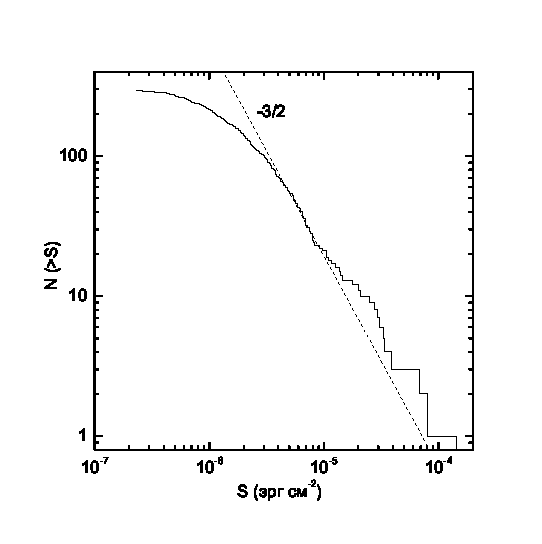
\includegraphics[height=0.45\textwidth]{glogNlogS_ru.eps}}
		\subfigure[]{\label{fig:logNlogPF}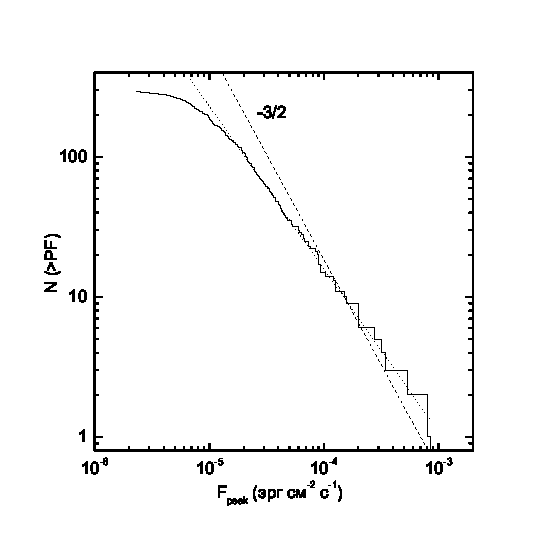
\includegraphics[height=0.45\textwidth]{glogNlogPF_ru.eps}}
	\end{center}
\caption{
    Интегральные распределения $\log N$--$\log S$~\subref{fig:logNlogS} и
    $\log N$--$\log F_\rmn{peak}$~\subref{fig:logNlogPF}.
    Пунктирная линия обозначает степенное распределение с показателем степени $-3/2$,
    ожидаемое для однородного расположения источников всплесков в Евклидовом пространстве.
    Штриховая линия на панели~\subref{fig:logNlogPF} показывает степенную аппроксимацию
    распределения $\log N$--$\log F_\rmn{peak}$ в диапазоне  
    $(0.2\textrm{--}1.5)\times 10^{-4}$~эрг~см$^{-2}$~с$^{-1}$, полученный степенной индекс
    равен $-1.16\pm0.01$ ($\chi^2_r = 1.2$).
    \label{fig:logNlogS_PF} }
\end{figure}
